\documentclass{article}

\usepackage{enumitem}
\usepackage{fancyhdr}
\usepackage{listings}
\usepackage{graphicx}
\usepackage[lastexercise]{exercise}   %add in noanswer
\usepackage{color}
% for exercise 


\definecolor{dkgreen}{rgb}{0,0.6,0}
\definecolor{gray}{rgb}{0.5,0.5,0.5}
\definecolor{mauve}{rgb}{0.58,0,0.82}


\lstset{frame=tb,
  language=Haskell,
  aboveskip=3mm,
  belowskip=3mm,
  showstringspaces=false,
  columns=flexible,
  basicstyle={\small\ttfamily},
  numbers=none,
  numberstyle=\tiny\color{gray},
  keywordstyle=\color{blue},
  commentstyle=\color{dkgreen},
  stringstyle=\color{mauve},
  breaklines=true,
  breakatwhitespace=true,
  tabsize=3
  }
\def\AnswerName{Solution to Exercise}

%% Change this for title information 
\newcommand\ExTitle{Functions}

\newcommand\fullExTitle{Exercises \\ \ExTitle }
\newcommand\footerExTitle{\ExTitle -\  Exercises and Solutions}

\pagestyle{fancy}
\fancyhead{} % clear all header fields
\renewcommand{\headrulewidth}{0pt} % no line in header area
\fancyfoot{} % clear all footer fields
\fancyfoot[LE,RO]{\thepage}           % page number in "outer" position of footer line
\fancyfoot[RE,LO]{\footerExTitle} % other info in "inner" position of footer line



\begin{document}
\begin{Huge}
	\begin{center}
	\fullExTitle
	\end{center}
\end{Huge}

\vspace{1cm}

\AtBeginExercise{\LARGE{\textbf{Basic Functions to start} }}
\begin{Exercise}
  Write a function named add1 that takes an Int and returns an Int that is one greater
than its input. For example, if we compute add1 5, we should get 6. If you want to
write a type signature for add1, it would be 
\begin{lstlisting}[language=Haskell]
add1 :: Int -> Int
\end{lstlisting} 

\end{Exercise}
\begin{Answer}
\begin{lstlisting}[language=Haskell]
add1 :: Int -> Int
add1 x = x+1  
\end{lstlisting}
\end{Answer}

\begin{Exercise}
Write a function: 
\begin{lstlisting}
   always0 :: Int->  Int
\end{lstlisting}   
The return value should always just be 0.
\end{Exercise}
\begin{Answer}
  \begin{lstlisting}[language=Haskell]
always0 :: Int -> Int
always0 _ = 0
  \end{lstlisting}
\textbf{Note:} This function could also be written (with a different type, i.e. no input argument) as 
\begin{lstlisting}[language=Haskell]
always0 :: Int
always0  = 0
    \end{lstlisting}
  \end{Answer}
  
\begin{Exercise}
  Write a function:
  \begin{lstlisting}
subtract' :: Int-> Int-> Int
  \end{lstlisting}   
  that takes two numbers (that is, Ints) and subtracts them.
\end{Exercise}
\begin{Answer}
  \begin{lstlisting}[language=Haskell]
    subtract' :: Int -> Int -> Int
    subtract' x y = x-y
  \end{lstlisting} 
  
  \end{Answer}
  
\begin{Exercise}
  Write a function:
  \begin{lstlisting}
    addmult :: Int-> Int -> Int-> Int
  \end{lstlisting}   
  that takes three numbers. Let’s call them p, q, and r. \textbf{addmult}  should add p and q together and then multiply the result by r.
\end{Exercise}

\begin{Answer}

\begin{lstlisting}[language=Haskell]
addmult :: Int -> Int -> Int -> Int
addmult x y z = (x+y) * z
  
\end{lstlisting}
  \end{Answer}

\vspace{1cm}
\pagebreak
\AtBeginExercise{\LARGE{\textbf{Conditionals}}}
\begin{Exercise}
Write a function 
\begin{lstlisting}
greaterThan0 :: Int -> String
\end{lstlisting}   
That returns the String "Yes!" if the number is greater than 0, and "No!" otherwise. 
\end{Exercise}
\begin{Answer}
  \begin{lstlisting}[language=Haskell]
greaterThan0 :: Int -> String
greaterThan0 n = if n>0 then "Yes" else "No!"
    
  \end{lstlisting}
  \end{Answer}

%   Write a function pushOut that takes a number and returns the number that is one step
% further from 0. That is, pushOut 3 is 4, pushOut (−10) is (−11), and pushOut 0 is 0.
% That last one is because we don’t know which direction to go! Note that, in Haskell,
% you always have to put parentheses around negative numbers

\begin{Exercise}
 Look at the function 
  \begin{lstlisting}
pushOut :: Int -> Int
  \end{lstlisting}   

  that takes a number and returns the number that is one step further from 0. 
  That is, 
  \begin{itemize}
    \item pushOut 3 is 4, 
    \item pushOut (-10) is (-11), and
    \item pushOut 0 is 0.
  \end{itemize}

That last one is because we don’t know which direction to go!.\\ \\


Write this function using 
\begin{enumerate}
  \item if .. then .. else  (call this pushOut)
  \item guarded equations    (call this pushOut')
\end{enumerate}
 
  \textbf{Remember} that, in Haskell, have to put parentheses around negative numbers
  \end{Exercise}

  \begin{Answer}
    \begin{enumerate}
      \item
      \begin{lstlisting}[language=Haskell]
pushOut :: Int -> Int
pushOut n  = if n > 0 then n+1 
            else if n < 0 then n-1
            else 0
          \end{lstlisting}

      \item  
      \begin{lstlisting}[language=Haskell]
pushOut' :: Int -> Int
pushOut' n  | n > 0     = n+1 
            | n < 0     = n-1
            | otherwise =  0
          \end{lstlisting}
    \end{enumerate}
   
    \end{Answer}

\begin{Exercise} 
Using library functions, define a function \\
\begin{lstlisting}
  halve :: [a] -> ([a], [a])
\end{lstlisting}
that splits an even-lengthed list into two halves. For example: 
\begin{center}
	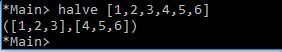
\includegraphics[width=8cm]{img/01.jpg}
\end{center}
\end{Exercise}
\begin{Answer}
\begin{lstlisting}[language=Haskell]
halve :: [a] -> ([a], [a]) 
halve xs = (take half xs, drop half xs) where 
       half = length xs `div` 2
\end{lstlisting}
\end{Answer}
%\item 
\begin{Exercise} 

Define a function \textbf{\textit{third}}\\
\begin{lstlisting}
  third :: [a] -> a
\end{lstlisting}
that returns the third element in a list that contains at least this many elements using:
\begin{enumerate}
	\item \textbf{\textit{head}} and \textbf{\textit{tail}};
	\item list indexing \textbf{\textit{!!}};
	\item pattern matching.
\end{enumerate}
\end{Exercise}
\begin{Answer}
\begin{lstlisting}
third :: [a] -> a
third xs = head (tail (tail xs)) 

third' :: [a] -> a
third' xs = xs !! 2

third'' :: [a] -> a
third'' (_:_:x:_) = x
\end{lstlisting}
\end{Answer}
\begin{Exercise} 

Consider a function \textbf{\textit{safetail}} that behaves in the same way as \textbf{\textit{tail}}, except that \textbf{\textit{safetail}} maps the empty list to the empty list, whereas tail gives an error in this case.  Define \textbf{\textit{safetail}} using:
\begin{enumerate}
	\item a conditional expression;
	\item guarded equations;
	\item pattern matching.
\end{enumerate}
\textbf{Hint:}  the library function \textbf{\textit{null}} :: [a] $->$ Bool can be used to test if a list is empty.
\end{Exercise}
\begin{Answer}
\begin{lstlisting}
safetail :: [a] -> [a]
safetail xs   =  if  null xs   then  [] else  tail xs

safetail' :: [a] -> [a]
safetail' xs | null xs  = []
             | otherwise = tail xs

safetail'' ::[a] -> [a]
safetail'' [] = []
safetail'' (_:xs) = xs
\end{lstlisting}
\end{Answer}
\begin{Exercise} 
In a similar way to \hspace {.5cm }\textbf{\textit{\&\hspace{-.5cm}\&}} \hspace{.5cm} in this section's slides, 
show how the disjunction operator \textbf{$\vert\vert$ } can be defined in three different ways using pattern matching.(Call it \textbf{myOr)}
\end{Exercise}
\begin{Answer}
\begin{lstlisting}[language=Haskell]
myor:: Bool -> Bool -> Bool
False  `myor` False = False
_ `myor` _          = True

myor':: Bool -> Bool -> Bool
False  `myor'` b = b
True `myor'` _   = True
\end{lstlisting}
\end{Answer}
\pagebreak
\begin{Exercise} 
Given the function with the following type :
\begin{lstlisting}[language=Haskell]
 lucky :: Integral a =>  a-> String
\end{lstlisting}
Write the function definition that returns the following strings given the following inputs:
\begin{enumerate}
 \item When input is 7, the output is the String "Lucky you.. Proceed directly to buy a lottery ticket.".
 \item When input is 13, the output is the String "You, sadly are quite unlucky. Do not, under any circumstances, invest money today."
 \item For any other input, the output is the String "Mmmm.... Can't really say...."
 \end{enumerate}
\end{Exercise}
\begin{Answer}
\begin{lstlisting}
-- (from Learn you a good Haskell)
lucky :: Integral a =>  a-> String
lucky 7 = "Lucky you.. Proceed directly to buy a lottery ticket."
lucky 13 = "You, sadly are quite unlucky. Do not, under any circumstances, invest money today "
lucky _ = "Mmmm.... Can't really say...."
\end{lstlisting}
\end{Answer}
\pagebreak
\begin{Exercise}
 Given the two (Prelude) functions \textbf{\textit{fst}} and \textbf{\textit{snd}} who return the first and second element of a 2-tuple respectively as in : 
\begin{lstlisting}[language=Haskell]
fst:: (a,b) -> a
fst(x, _) = x
snd :: (a,b) -> b
snd(_, y) = y
\end{lstlisting}
Write similar functions  - first, second and third who return the first, second and third element of a three tuple. 
\begin{lstlisting}
second (2,4,'e') = 4
\end{lstlisting}
\end{Exercise}
\begin{Answer}
\begin{lstlisting}
fst':: (a,b,c) -> a
fst'(x, _, _) = x
snd' :: (a,b,c) -> b
snd'(_, y,_) = y
thrd' :: (a,b,c) -> c
thrd'(_, _,z) = z
\end{lstlisting}
\end{Answer}
\pagebreak
\AtBeginExercise{\LARGE{\textbf{The next two  questions are optional}}}
\begin{Exercise} 

 The \textbf{\textit{Luhn Algorithm}} is used to check bank card numbers for simple errors such as mistyping a digit and proceeds as follows: 
\begin{itemize}
	\item consider each digit as a separate number;
	\item moving left, double every other number from the second last;
	\item subtract 9 from each number that is now greater than 9;
	\item add all the resulting numbers together;
	\item if the total is divisible by 10, the card number is valid.
\end{itemize}
Note that the rightmost digit is the check digit. 
Define a function 
\begin{lstlisting}
   luhnDouble :: Int -> Int 
\end{lstlisting}
that doubles the a digit and subtracts 9 if the number is greater than 9. For example 
\begin{center}
	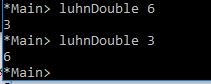
\includegraphics[width=8cm]{img/02.jpg}
\end{center}
Using \textbf{\textit{luhnDouble}} and the integer remainder function \textbf{\textit{mod}}, define a function 
\begin{lstlisting}[language=Haskell]
    luhn :: Int -> Int-> Int-> Int-> Bool
\end{lstlisting}


that decides if a four digit number is valid. For example:
\begin{center}
	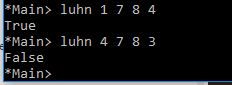
\includegraphics[width=8cm]{img/03.jpg}
\end{center}
\end{Exercise}
\pagebreak
\begin{Answer}
(From Hutton) 
\begin{lstlisting}[language=Haskell]
luhnDouble :: Int -> Int
luhnDouble x = if (x*2> 9) then x*2-9 else x*2

luhn :: Int -> Int -> Int -> Int -> Bool
luhn a b c d = (a' + b + c'+ d ) `mod` 10 == 0 where
       a' = luhnDouble a
       c' = luhnDouble c
\end{lstlisting}
\end{Answer}
\begin{Exercise}
Using the same definition of the luhn algorithm and remembering that the rightmost digit is the check digit, write a function 
\begin{lstlisting}[language=Haskell]
luhnGetCheck:: Int -> Int-> Int-> Int
\end{lstlisting}
that, given the leftmost three digits as per the previous example, calculates the check digit. 
For example 
\begin{center}
	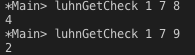
\includegraphics[width=8cm]{img/04.png}
\end{center}

\end{Exercise}
\begin{Answer}
(From Hutton) 
\begin{lstlisting}[language=Haskell]
luhnGetCheck :: Int-> Int -> Int -> Int
luhnGetCheck a b c = (10 - (luhnSum `mod` 10)) `mod` 10   where  
                      -- seccond `mod` to check for 10
       luhnSum = luhnDouble a + b + luhnDouble c 

\end{lstlisting}
And alternative from Elijah Hartvigsen (thanks Elijah!)
\begin{lstlisting}[language=Haskell]
    getCheckLuhn x y z = if luhnNum == 10 then 0 else luhnNum where
      luhnNum = 10 - partialSum `mod` 10
      partialSum = luhnDouble x + y + luhnDouble z
  \end{lstlisting}
\end{Answer}
% Uncomment this for the Answers
% \newpage
% \begin{Huge}
% \begin{center}
% Solutions
% \end{center}
% \end{Huge}
% \shipoutAnswer
\end{document}